
\begin{figure}
\center

	\begin{subfigure}[t]{0.22\textwidth}
		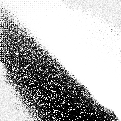
\includegraphics[width=\textwidth]{images/findings/experiments/randomization/strats/hand_max_min.png}
		\caption{\handmaxmin}
	\end{subfigure}
	~
	\begin{subfigure}[t]{0.22\textwidth}
		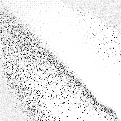
\includegraphics[width=\textwidth]{images/findings/experiments/randomization/strats/hand_max_avg.png}
		\caption{\handmaxavg}
	\end{subfigure}
	~
	\begin{subfigure}[t]{0.22\textwidth}
		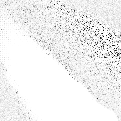
\includegraphics[width=\textwidth]{images/findings/experiments/randomization/strats/hand_max_med.png}
		\caption{\handmaxmed}
	\end{subfigure}
	~
	\begin{subfigure}[t]{0.22\textwidth}
		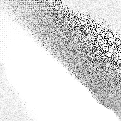
\includegraphics[width=\textwidth]{images/findings/experiments/randomization/strats/hand_max_poss.png}
		\caption{\handmaxposs}
	\end{subfigure}

	\begin{subfigure}[t]{0.22\textwidth}
		
\includegraphics[width=\textwidth]{images/findings/experiments/randomization/strats/crib_min_avg.png}
		\caption{\cribminavg}
	\end{subfigure}
	~
	\begin{subfigure}[t]{0.22\textwidth}
		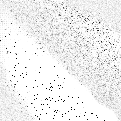
\includegraphics[width=\textwidth]{images/findings/experiments/randomization/strats/pegging_max_avg_gained.png}
		\caption{\peggingmaxavggained}
	\end{subfigure}
	~
	\begin{subfigure}[t]{0.22\textwidth}
		
\includegraphics[width=\textwidth]{images/findings/experiments/randomization/strats/pegging_max_med_gained.png}
		\caption{\peggingmaxmedgained}
	\end{subfigure}
	~
	\begin{subfigure}[t]{0.22\textwidth}
		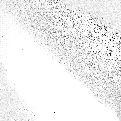
\includegraphics[width=\textwidth]{images/findings/experiments/randomization/strats/pegging_min_avg_given.png}
		\caption{\peggingminavggiven}
	\end{subfigure}

\caption{
	All final strategies for an agent which had its randomization strategy fixed
	to choose the combination of cards corresponding to the maximum value in
	the \pvec\ vector and with a chance of selecting at uniform random.
	These graphs are for when the agent is playing as the dealer.
}
\label{fig:expts-rand-strats}
\end{figure}
